 \chapter{Results}
 
 \section{Mesh movement}
 
 We present a case of rotation of an interior object inside a far-field boundary using interpolation methods. We show results for a 60-degree rotation in case of DGM (fig. \ref{fig:qin-60-dgm}), RBF (fig. \ref{fig:qin-60-rbf}) and DG-RBF2 (fig. \ref{fig:qin-60-dgrbf2}) methods. Note that DGRBF2 refers to the interpolation of rotation angles by DGRBF. The case has been referred from Wang \emph{et. al.} \cite{mm:dgrbf}. Figure \ref{fig:qin-orig} shows the un-deformed mesh.
 
 \begin{figure}
 	\centering
 	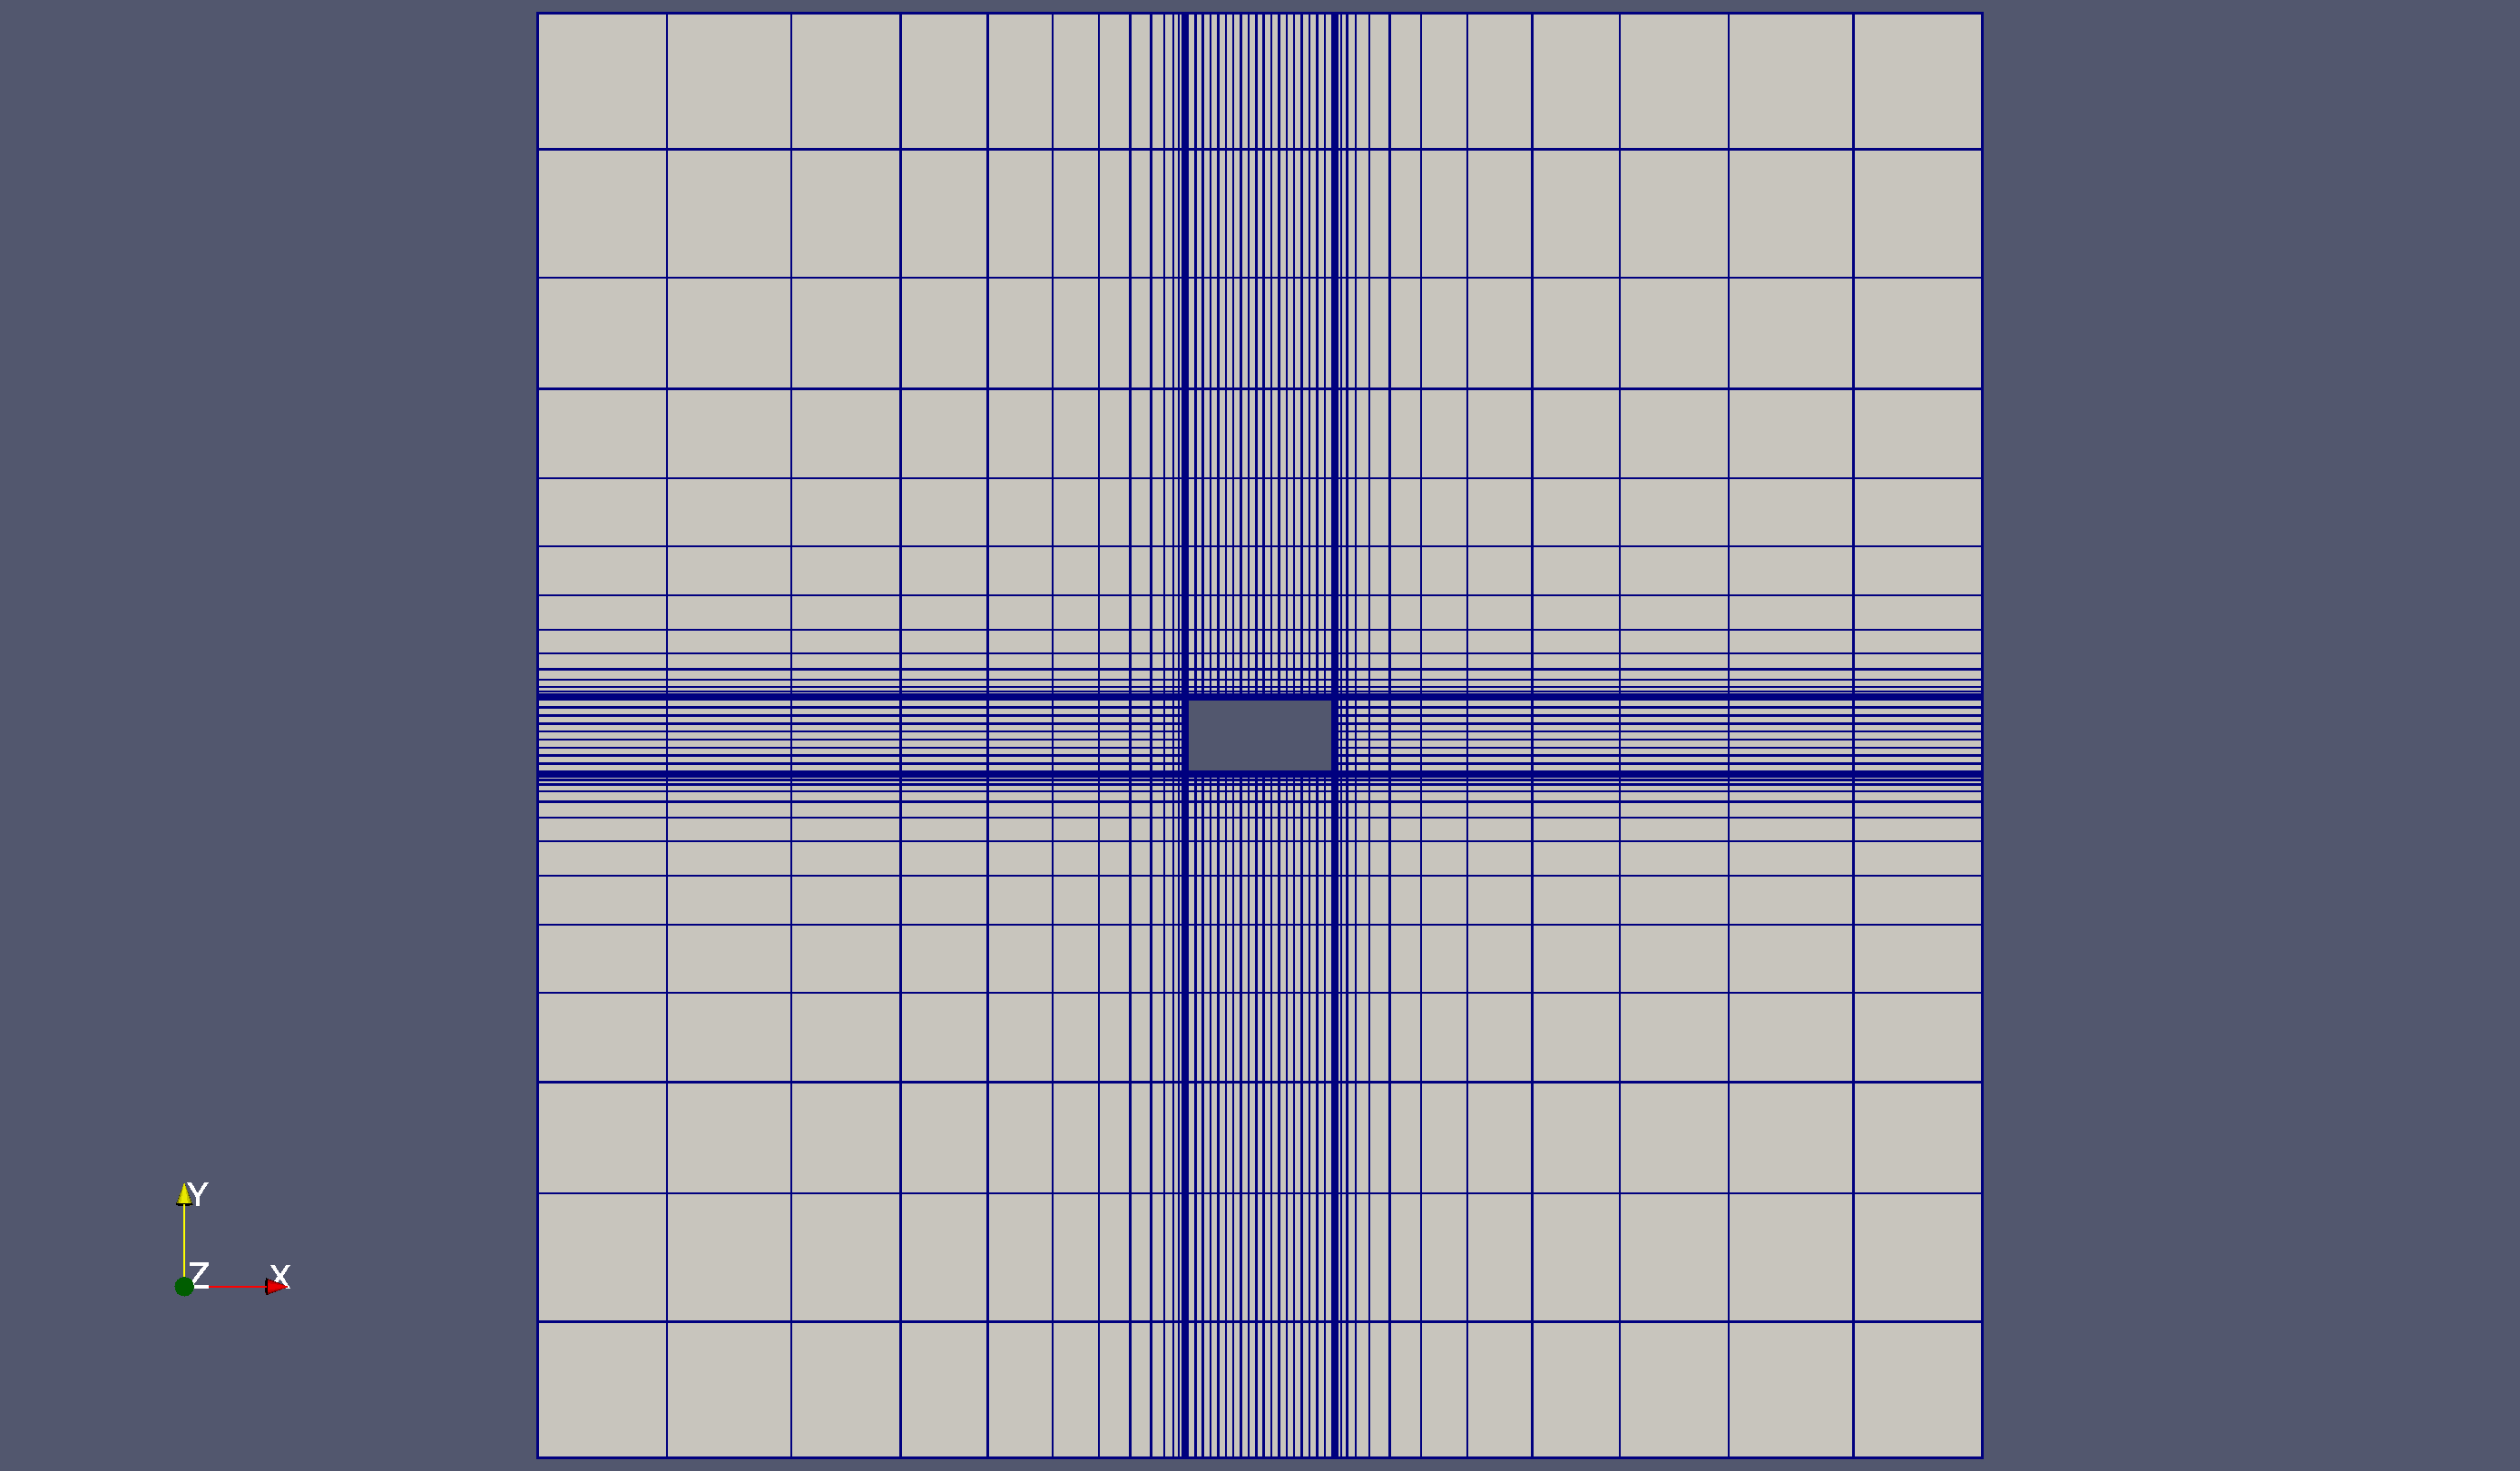
\includegraphics[scale=0.25]{qin-orig-mesh.pdf}
 	\caption{Original mesh}
 	\label{fig:qin-orig}
 \end{figure}
 
 \begin{figure}
 	\centering
 	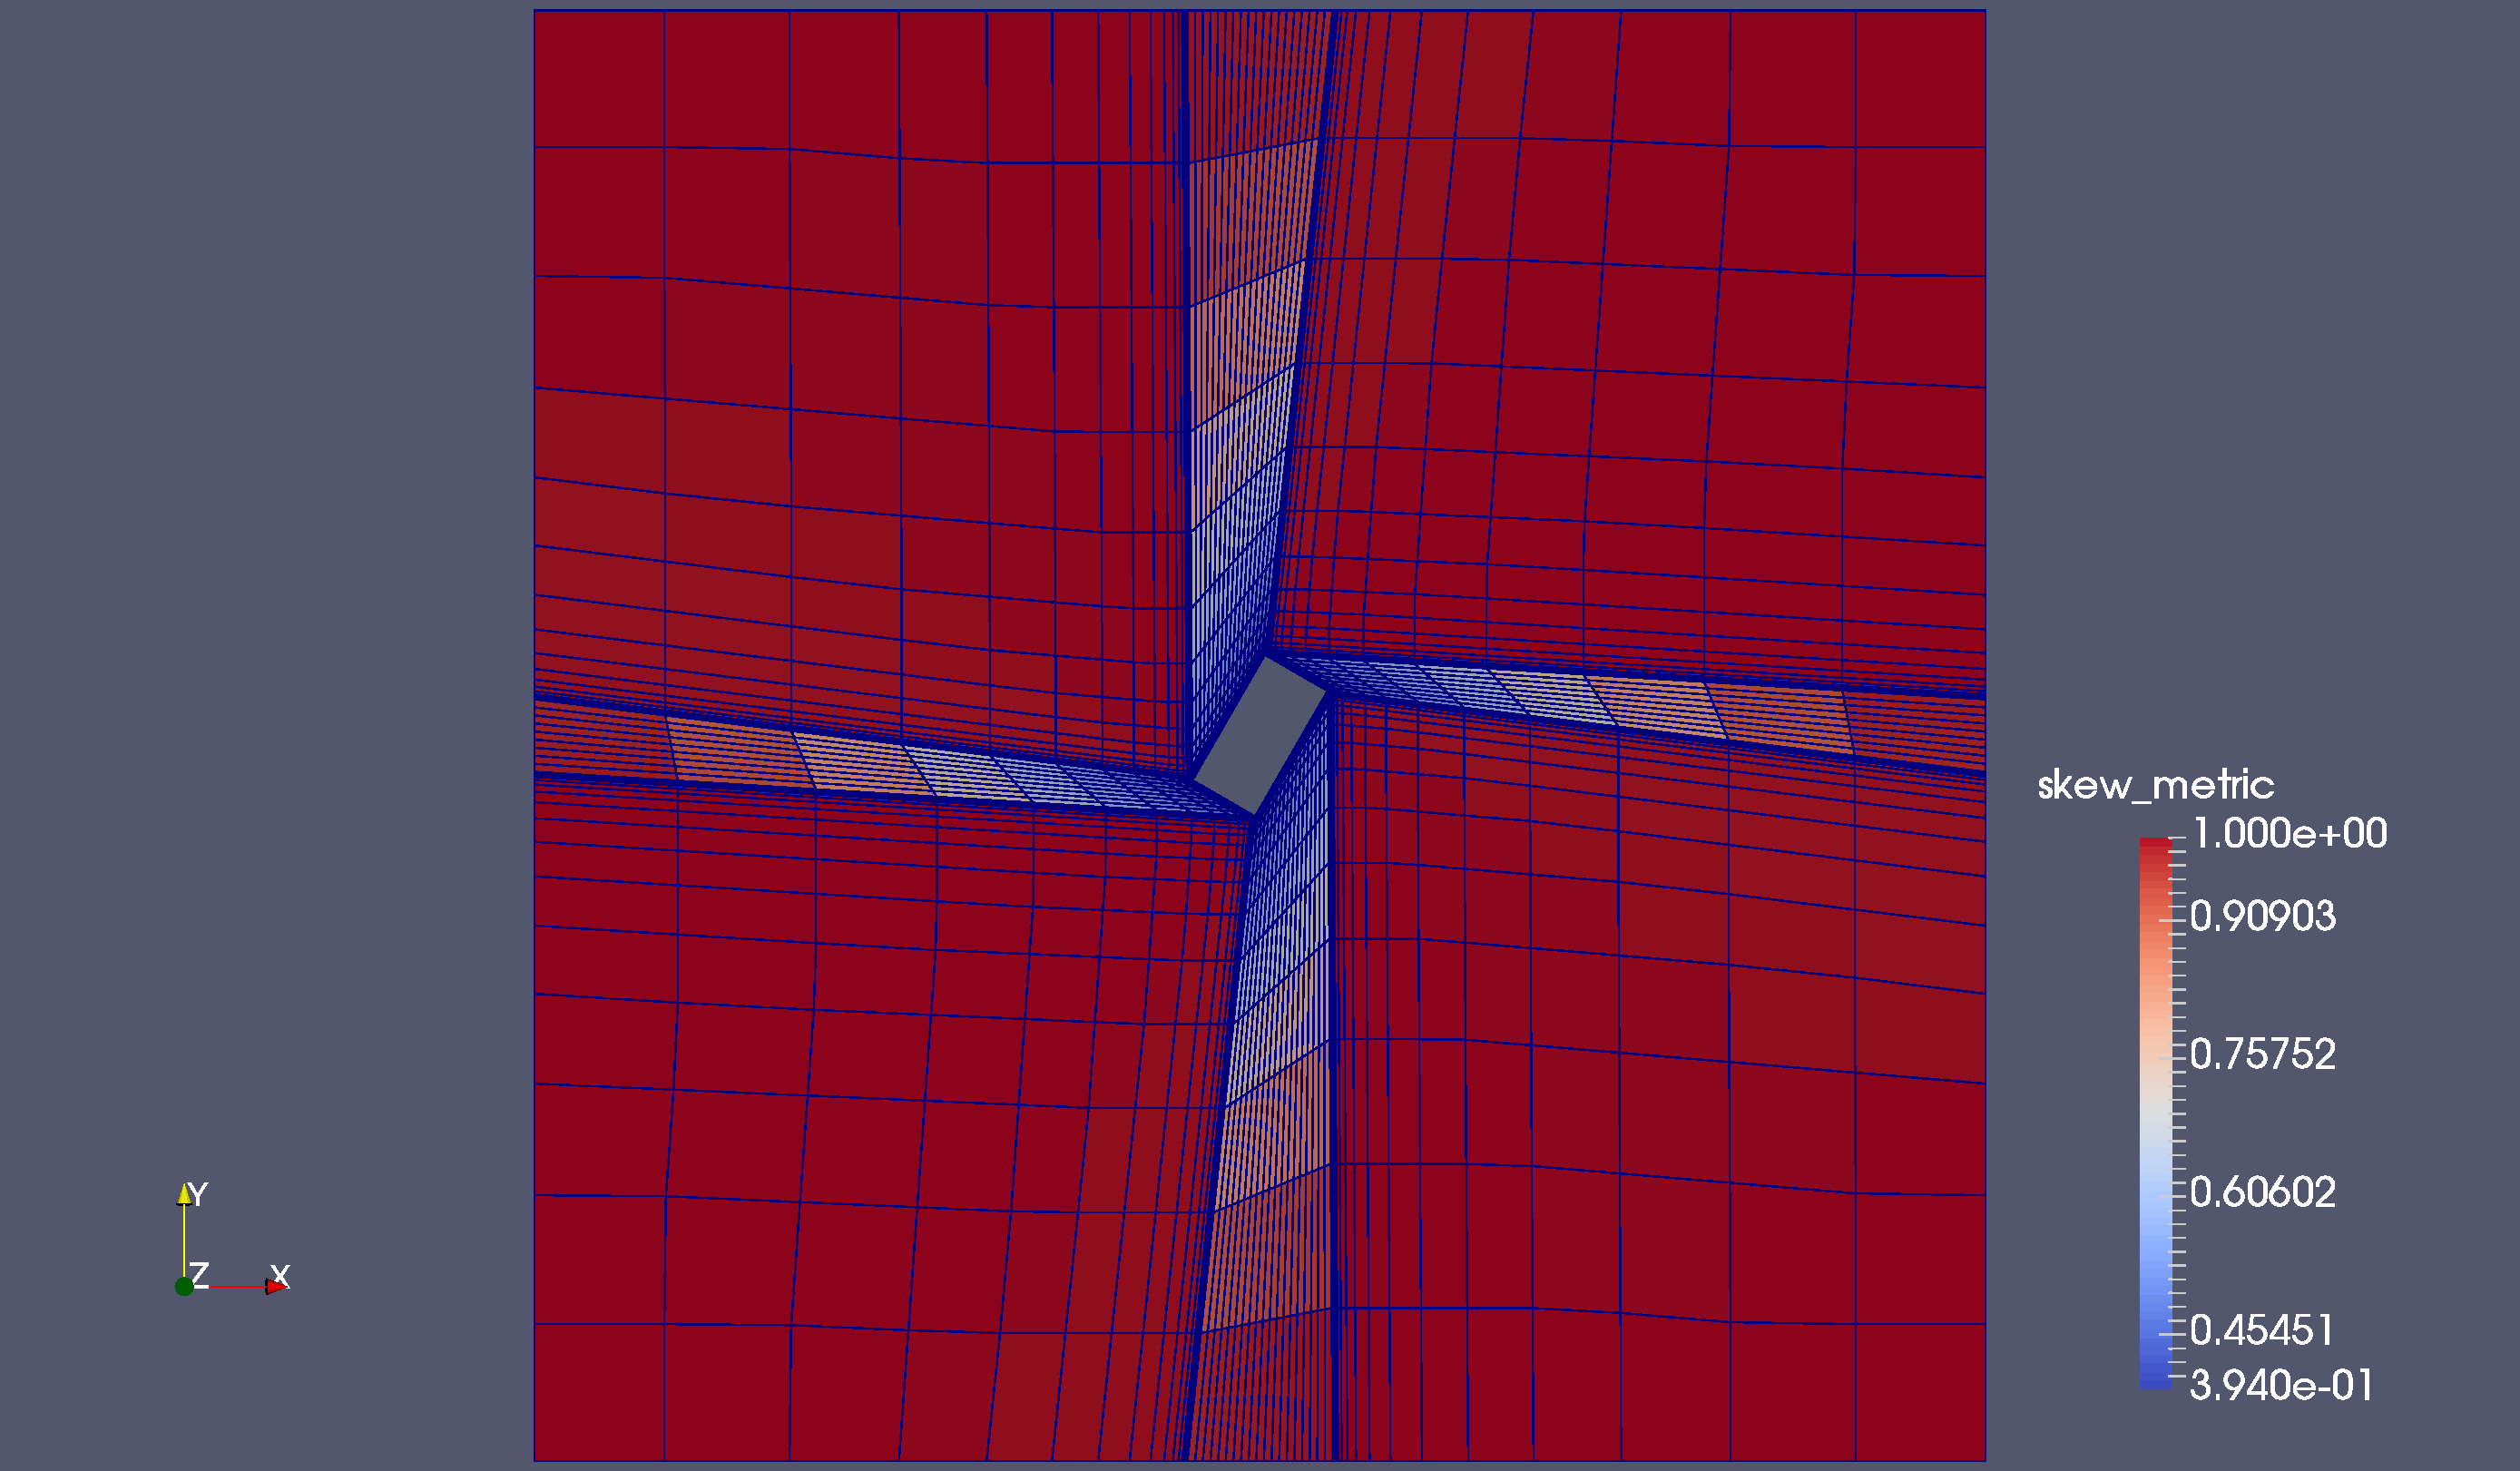
\includegraphics[scale=0.25]{qin-60-dgm-quality.pdf}
 	\caption{60 degrees rotation by DGM}
 	\label{fig:qin-60-dgm}
 \end{figure}
 
 \begin{figure}
 	\centering
 	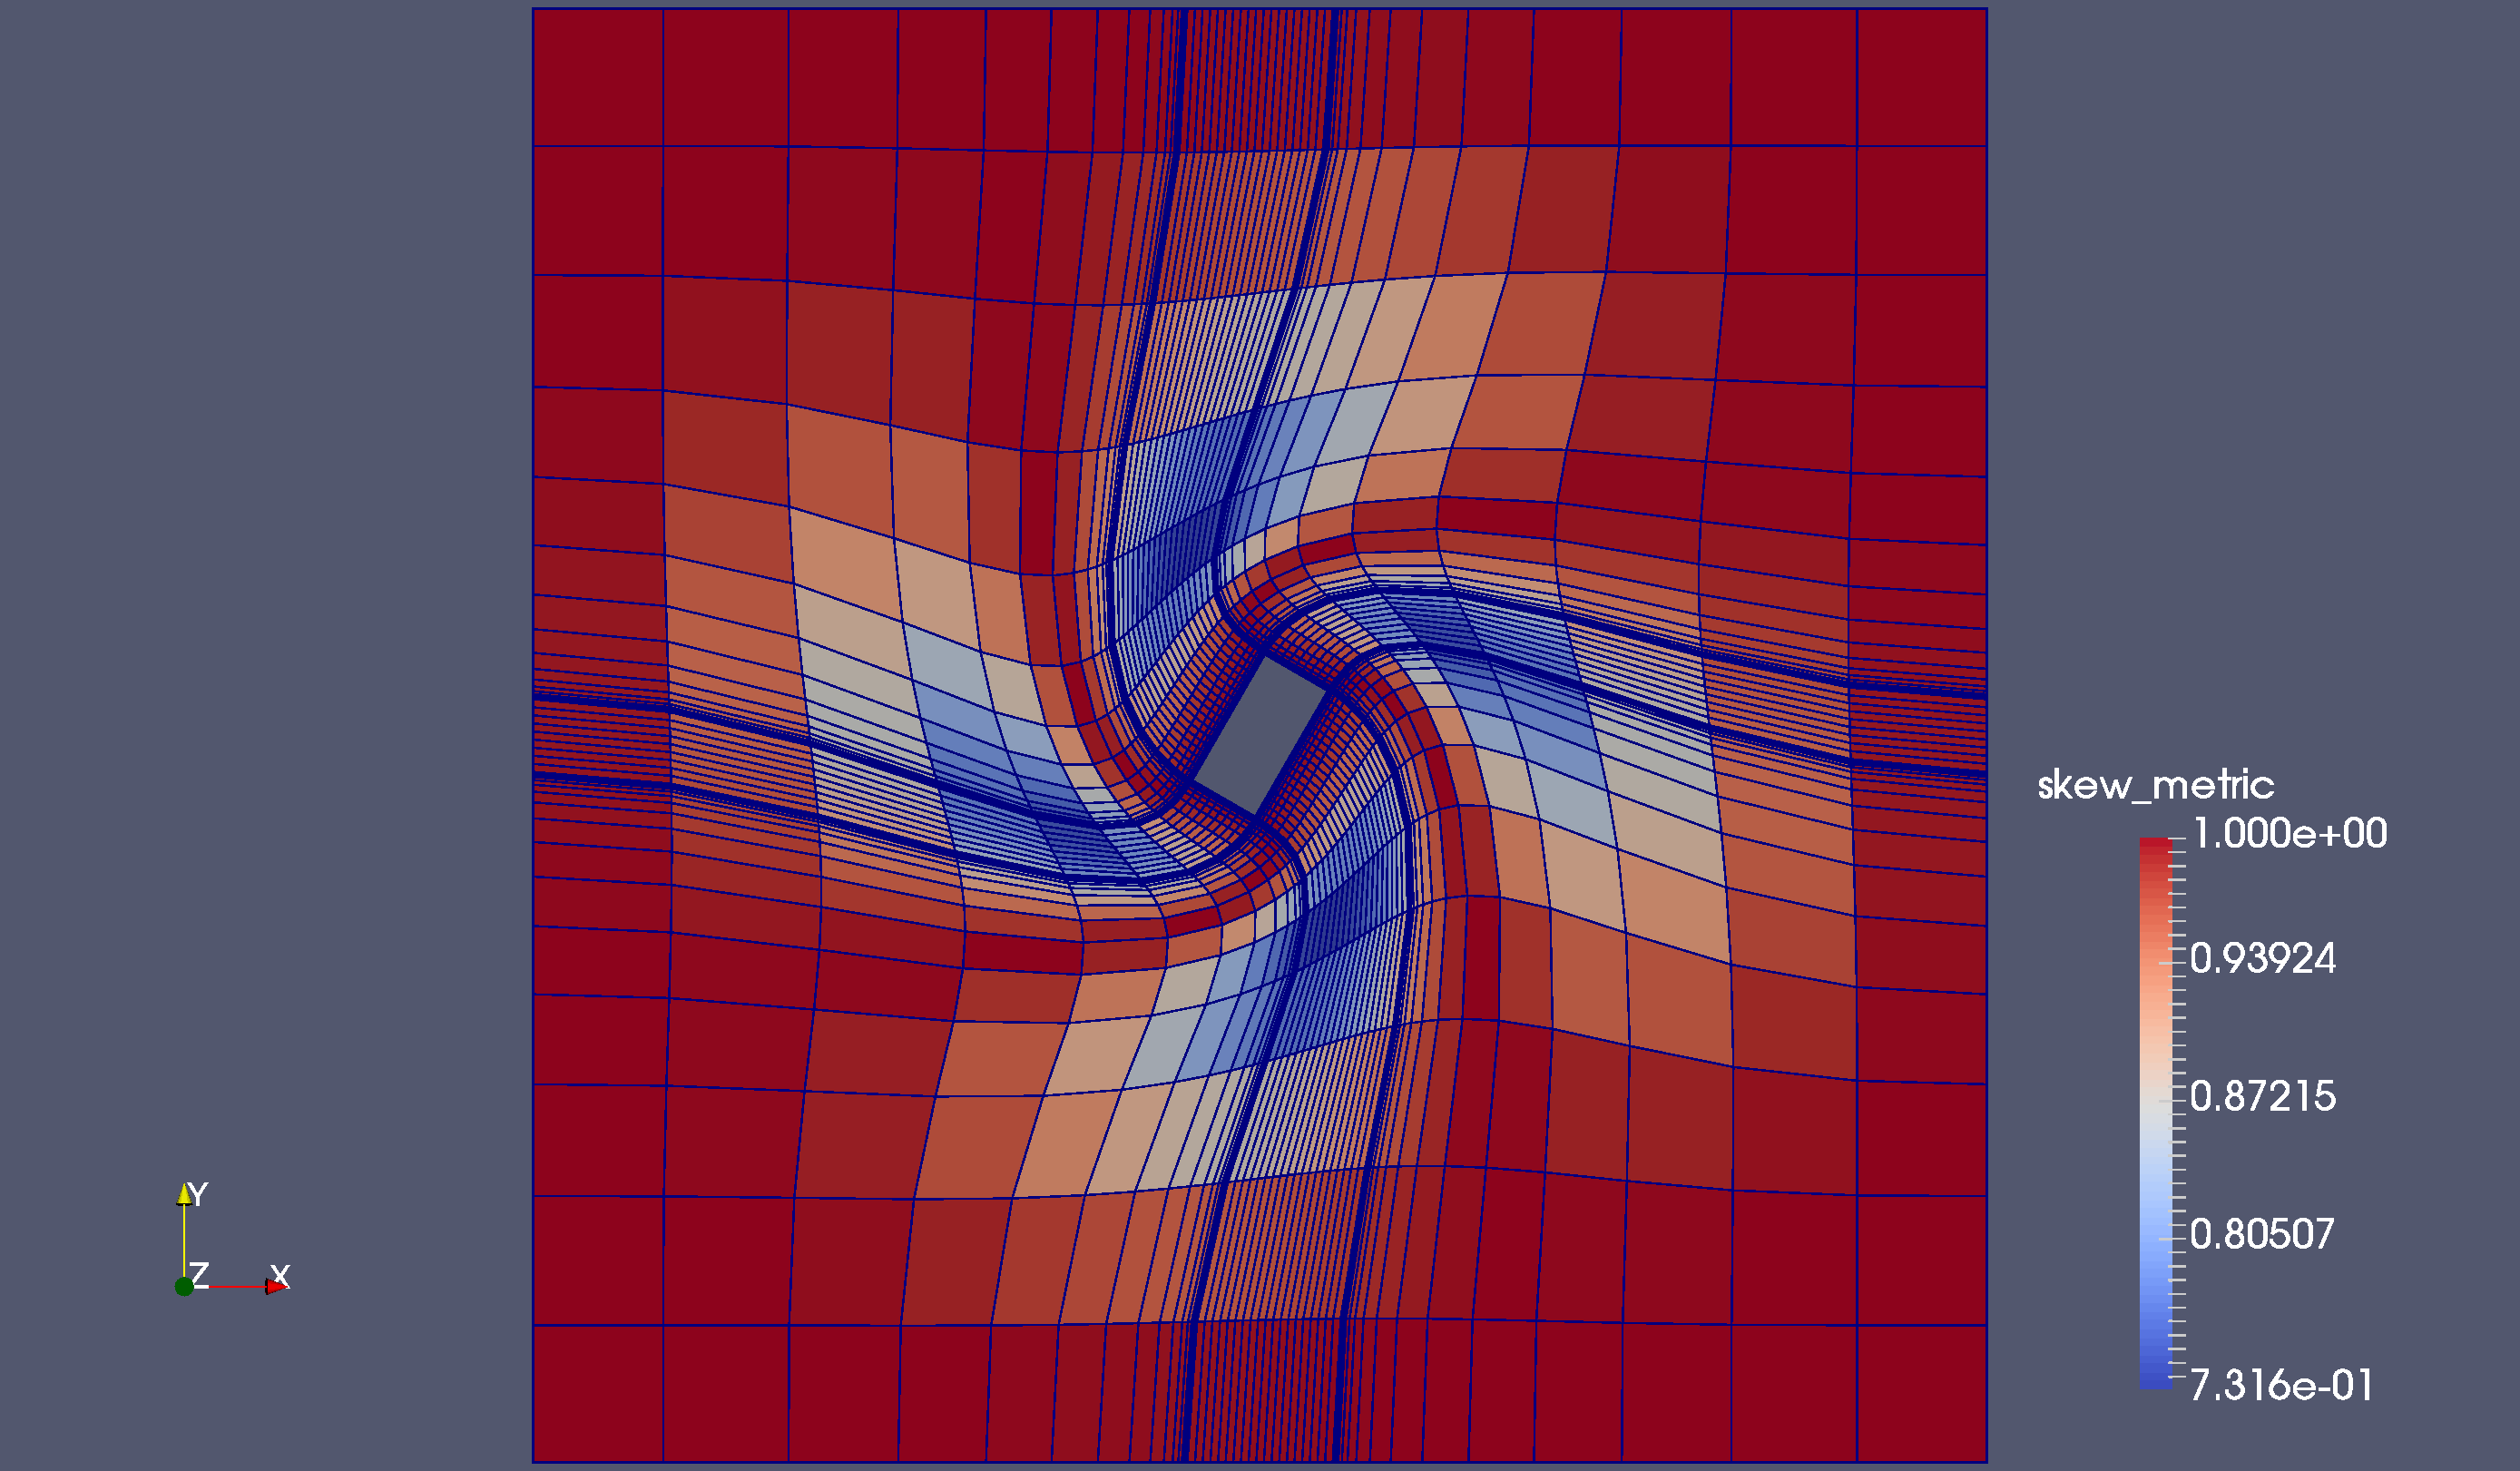
\includegraphics[scale=0.25]{qin-60-rbf-quality.pdf}
 	\caption{60 degrees rotation by RBF}
 	\label{fig:qin-60-rbf}
 \end{figure}
 
 \begin{figure}
 	\centering
 	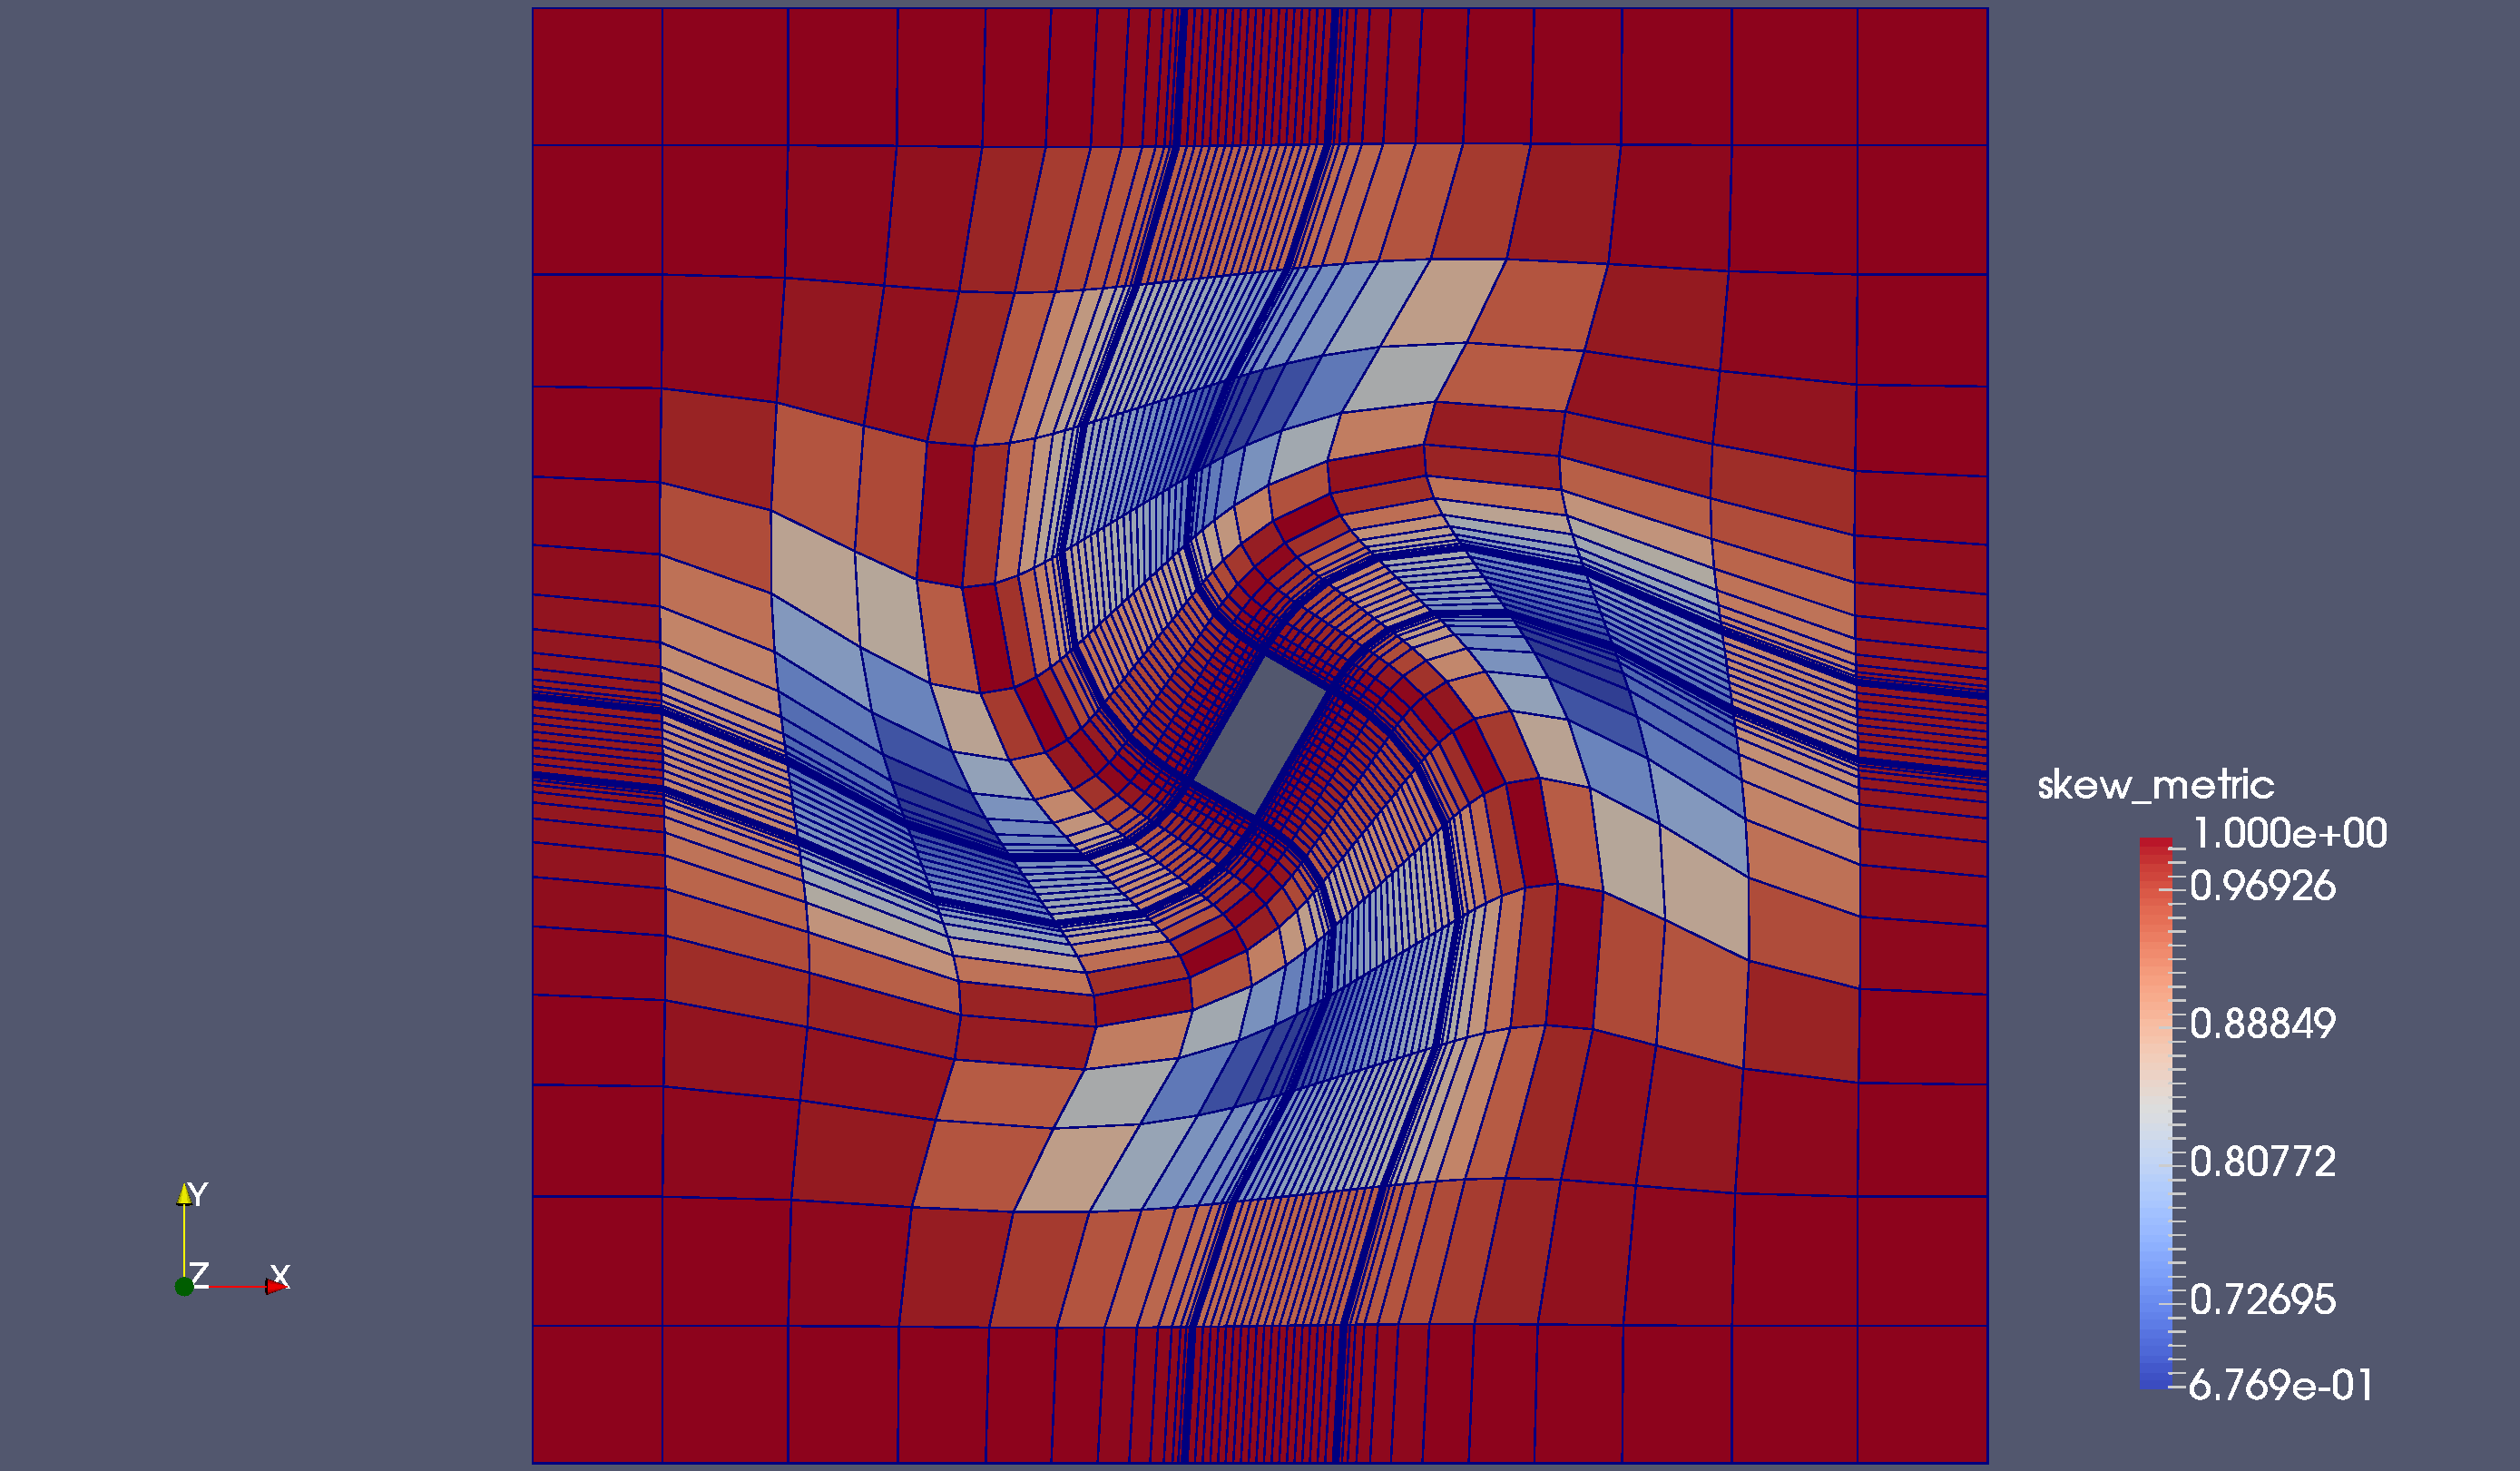
\includegraphics[scale=0.25]{qin-60-dgrbf2-quality.pdf}
 	\caption{60 degrees rotation by DGRBF2}
 	\label{fig:qin-60-dgrbf2}
 \end{figure}
 
 We note that the RBF and DGRBF2 methods can handle the rotation case quite well. The stretched, fine elements near the inner boundaries are well-preserved, while the elements further in the interior, which are larger and can thus take more deformation, are distorted somewhat. Though RBF gives slightly better mesh quality than DGRBF2 for this amount of rotation, RBF takes 1.926 seconds of total CPU time (using conjugate gradient solver), while DGRBF2 takes only 0.08 seconds of total CPU time. Further, shown in figure \ref{fig:qin-dgrbf2-120} is a case of extreme rotation of 120 degrees, which DGRBF2 solves while maintaining mesh validity. None of the other methods are able to do this. RBF has been found to give valid meshes upto about 110 degrees of rotation.
 \begin{figure}
 	\centering
 	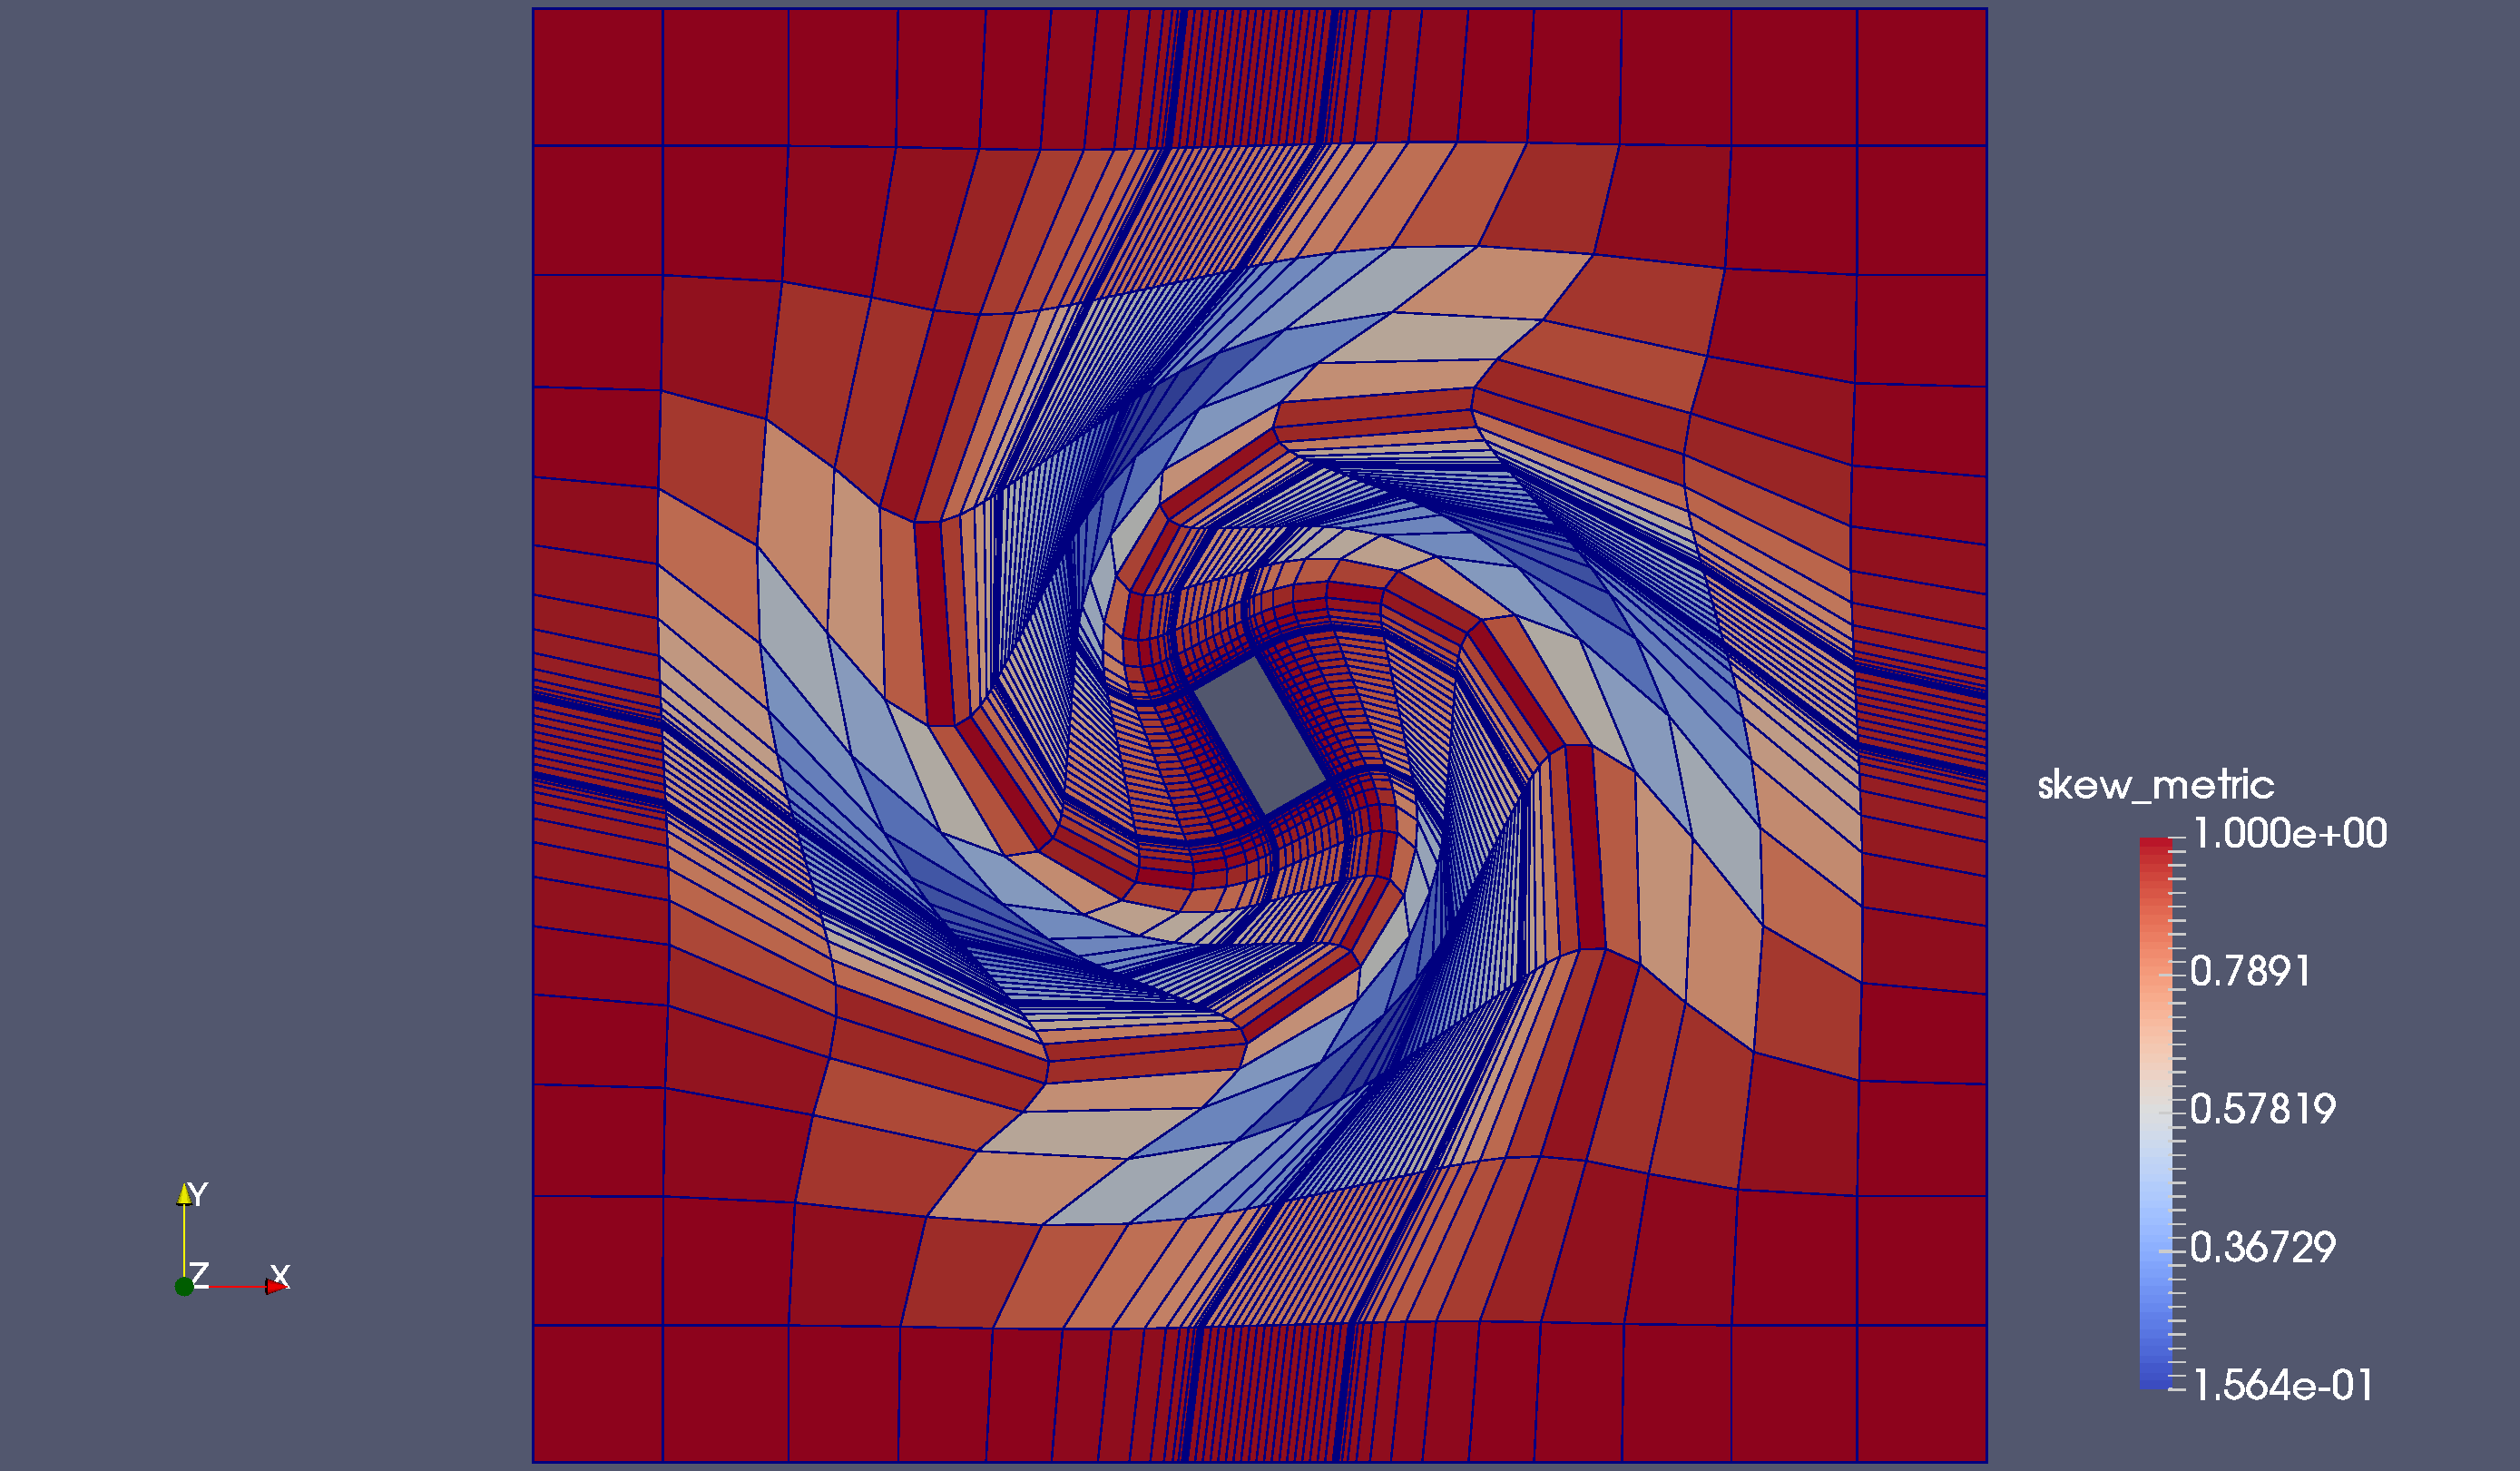
\includegraphics[scale=0.25]{qin-120-quality-withmesh.pdf}
 	\caption{Large rotational motion carried out by DGRBF2}
 	\label{fig:qin-dgrbf2-120}
 \end{figure}
 
 While solving certain problems with the pure RBF method, we find that the linear system to be solved is sometimes quite ill-conditioned, depending upon the mesh. However, in some of the cases that we worked on (such as curved mesh generation of hybrid meshes for viscous simulations of airfoils), sparse direct methods are capable of solving the system efficiently and effectively. This is likely to hold true in general as the systems to be solved will usually not be very large (having size of the number of boundary nodes).
 
 \section{Generation of curved meshes}
 
 Curved meshes for various standard viscous flow test cases have been generated with the method described in the previous section. These include flow past NACA0012 airfoil, flow through a bump channel and flow past a multi-element airfoil. Out of these, the mesh for the multi-element airfoil case is a truly unstructured mesh; the others are structured meshes which we first convert to unstructured format.
 
 The validity, and to some extent quality, of the generated mesh is established by computing the minimum scaled Jacobian determinant for each element. If the minimum value of the Jacobian determinant is zero or negative, the element is considered invalid. This is done as a post-processing step using the plugin `AnalyseCurvedMesh' available in Gmsh \cite{gmsh}. The quantity computed by this plugin is given as
 \begin{equation} 
 m_i = \frac{\inf_{\mathbf{x}\in\Omega_i}\det \mathbf{J}(\mathbf{x})}{\det \mathbf{J_l}_i},
 \end{equation}
 where $\mathbf{J}$ is the Jacobian matrix of the transformation of a reference element to the curved physical element, and $\mathbf{J_l}$ is the Jacobian of the transformation of the reference element to the linear (straight) physical element. $\Omega_i$ represents the \emph{i}th element.
 
 Here, we present results of 2D curved mesh generation in case of a multi-element airfoil. The mesh has triangular elements. It is meant for viscous flow computations and thus has highly stretched, thin elements near the wing boundaries. In this case, if the interior nodes are not moved properly, invalid elements result. In the figures, we compare curved meshes generated by isotropic linear elasticity and RBF interpolation. Both problems are solved using a Jacobi-preconditioned CG solver. Linear elasticity uses a Young's modulus $E$ of $1\times 10^6$ Pa and a Poisson's ratio of 0.4, though it is observed that the particular values do not influence the outcome much. A number of values over the range 1.0 to $1.0 \times 10^{10}$ were tried for $E$. RBF interpolation uses a support radius of 0.04 (for reference, the chord length of the wing is approximately 18.3).
 
 \begin{figure}
 	\centering
 	\includegraphics[width=300.0pt]{3compblack}
 	\caption{Mesh of multi-element airfoil. The little box shows approximately the region which is magnified in the figures that follow.}
 \end{figure}
 
 \begin{figure}
 	\centering
 	\subfloat{
 		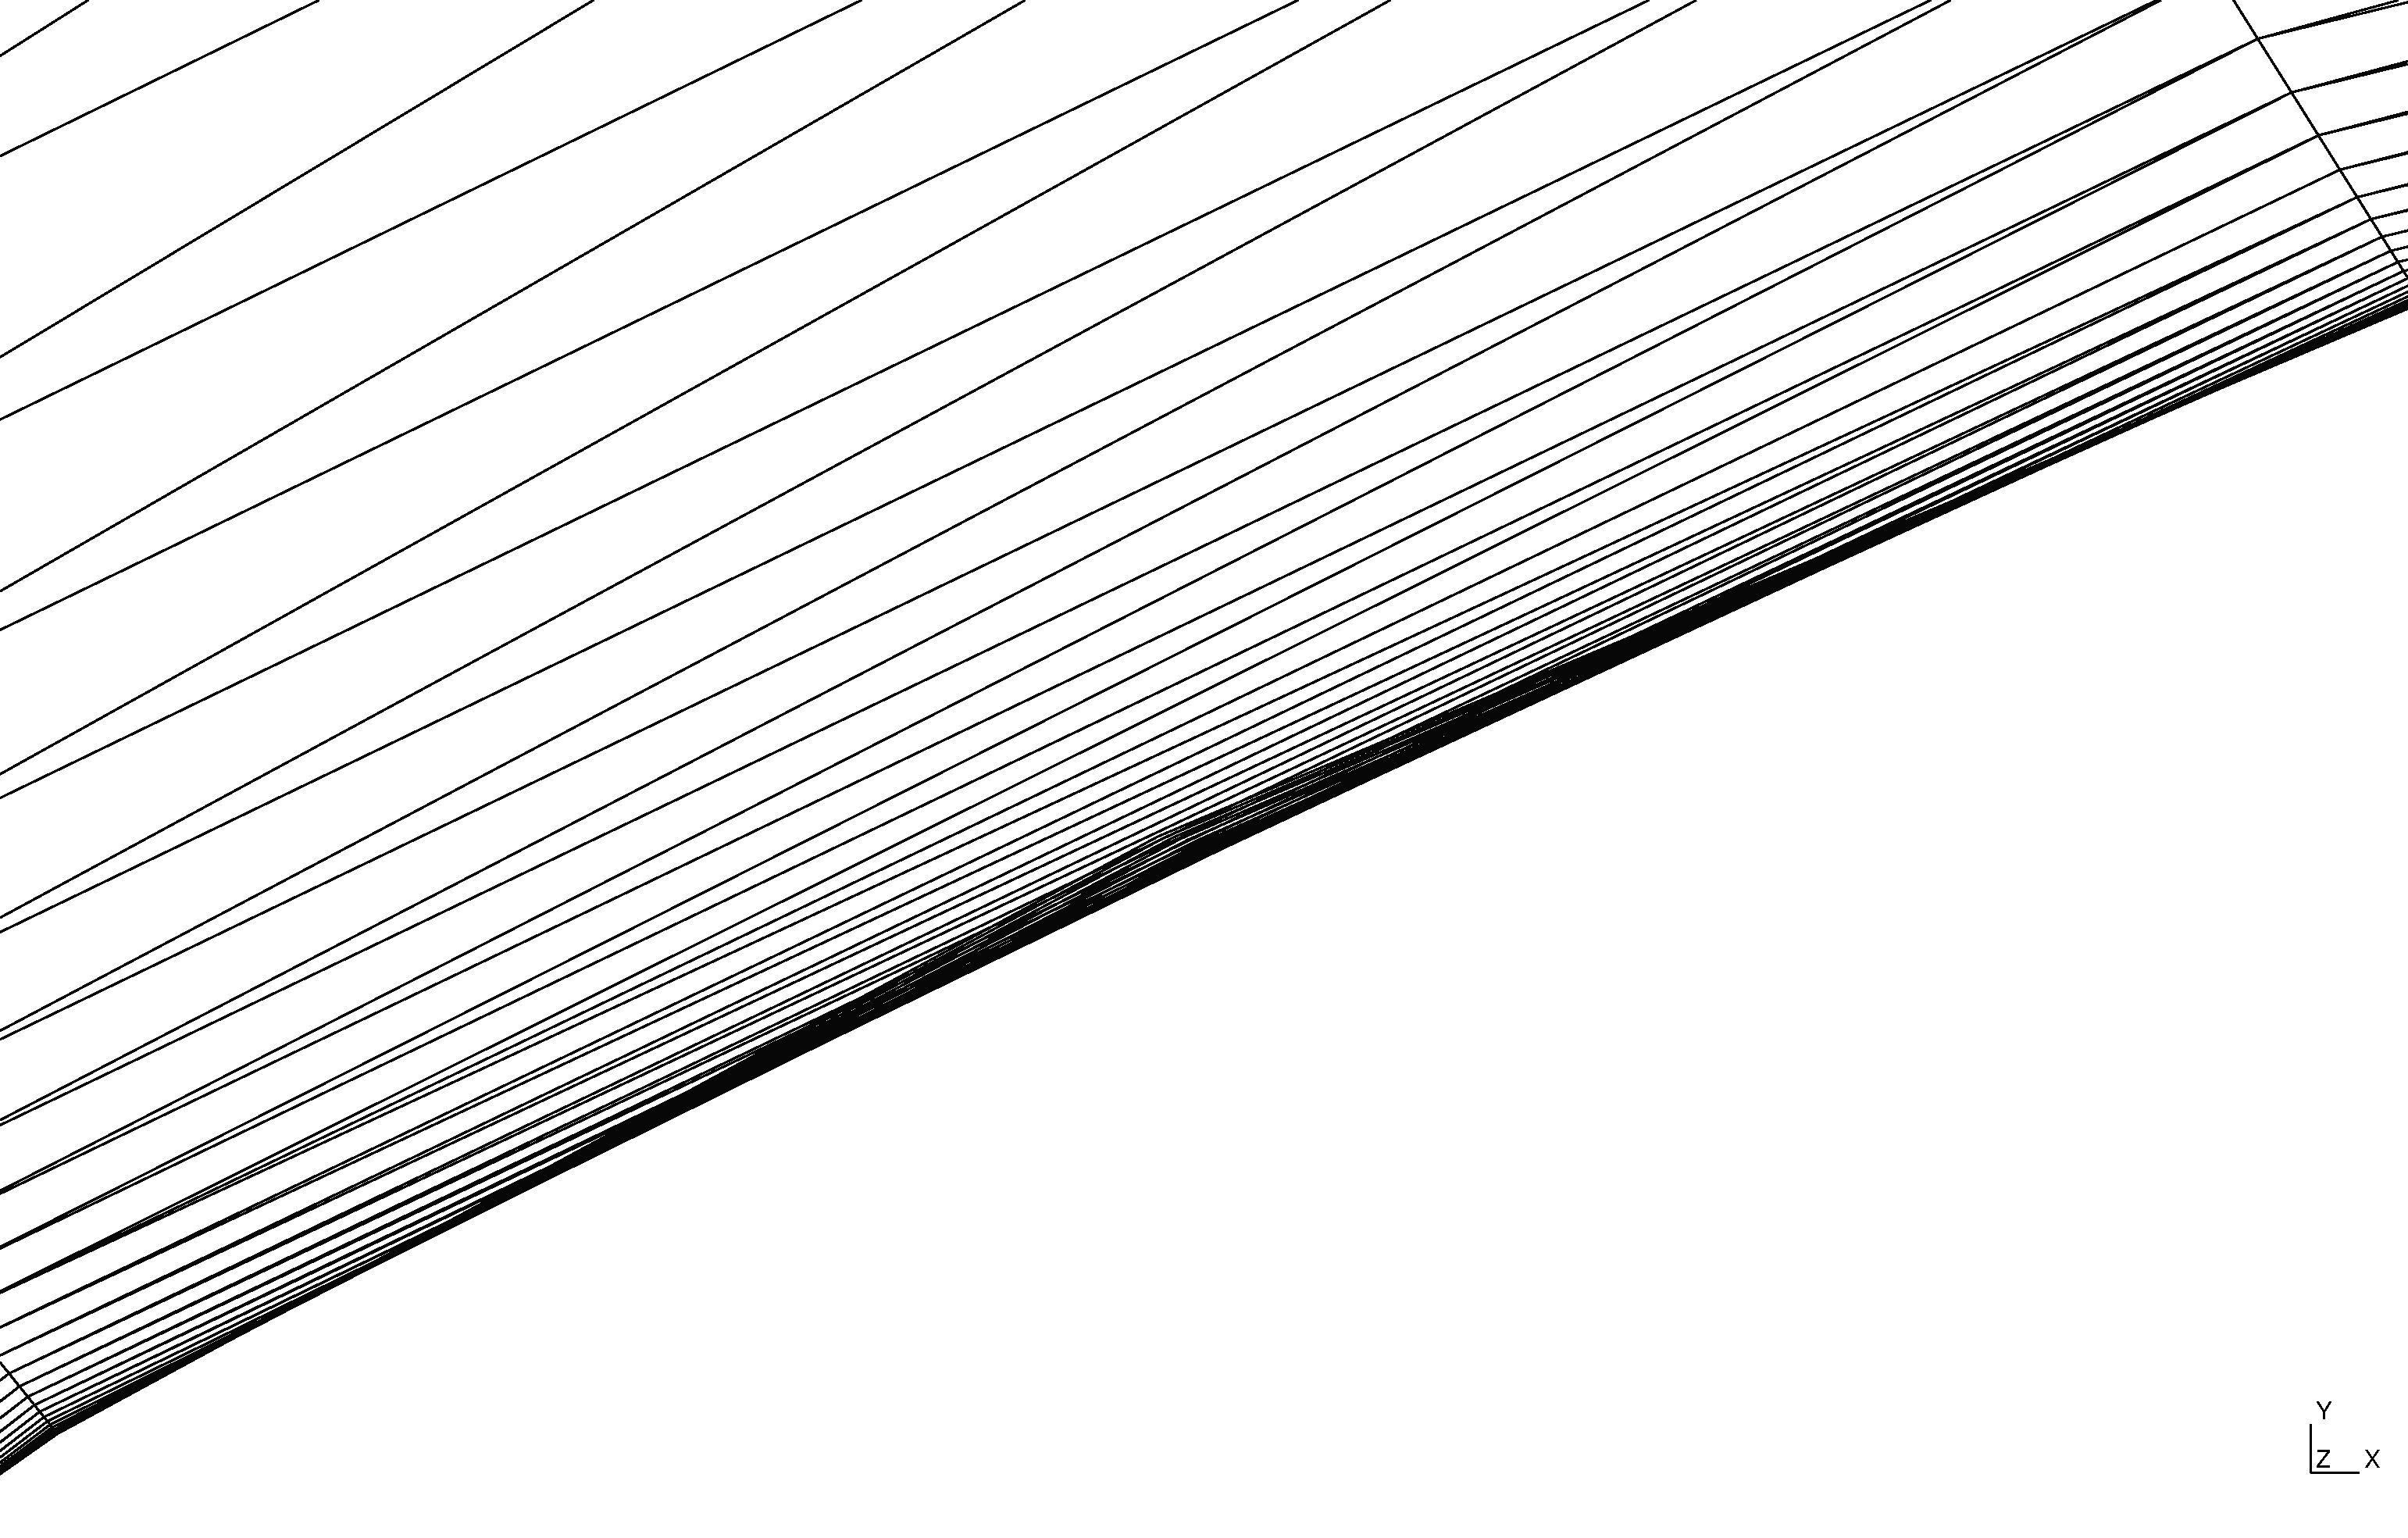
\includegraphics[width=200.0pt]{3comp-elast-zoomedblk.pdf}
 	}
 	\subfloat{
 		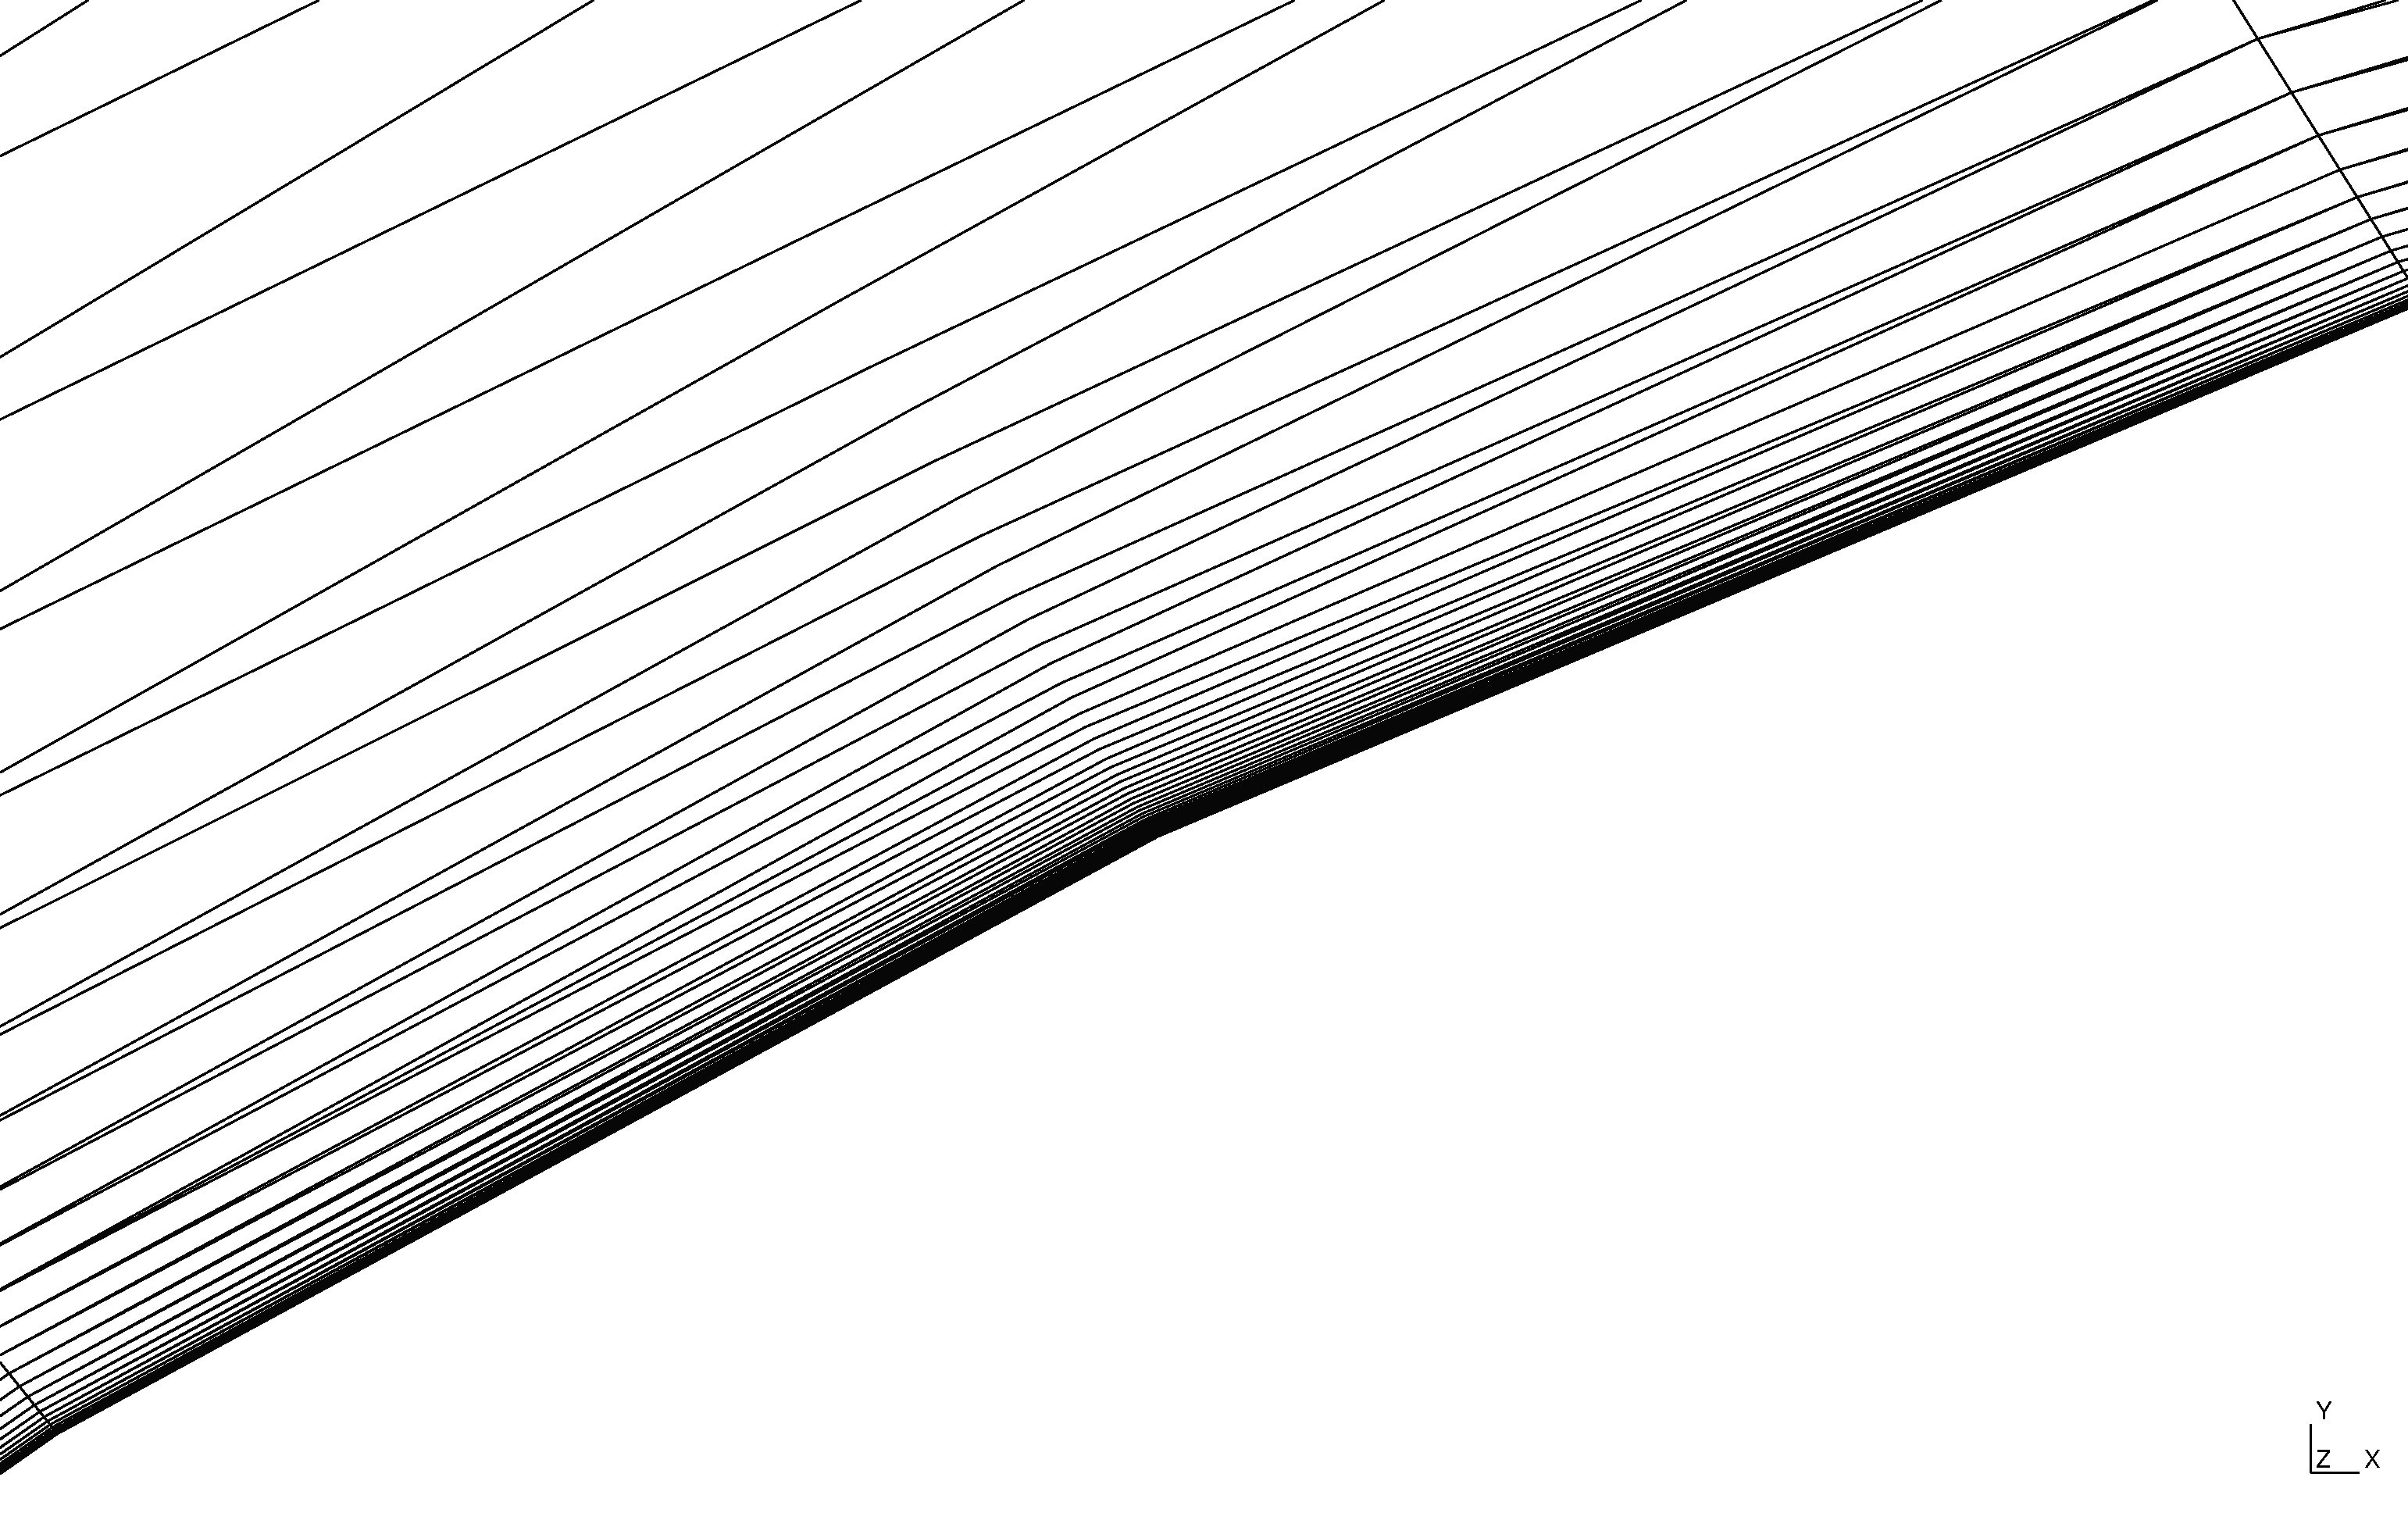
\includegraphics[width=200.0pt]{3comp-rbf-zoomedblk.pdf}
 	}
 	\caption{Portion of quadratic viscous mesh for multi-element airfoil, showing a boundary face in the flap, generated by linear elasticity (left) and RBF (right) methods.}
 	\label{fig:tangled1}
 \end{figure}
 
 \begin{figure}[!h]
 	\centering
 	\subfloat{
 		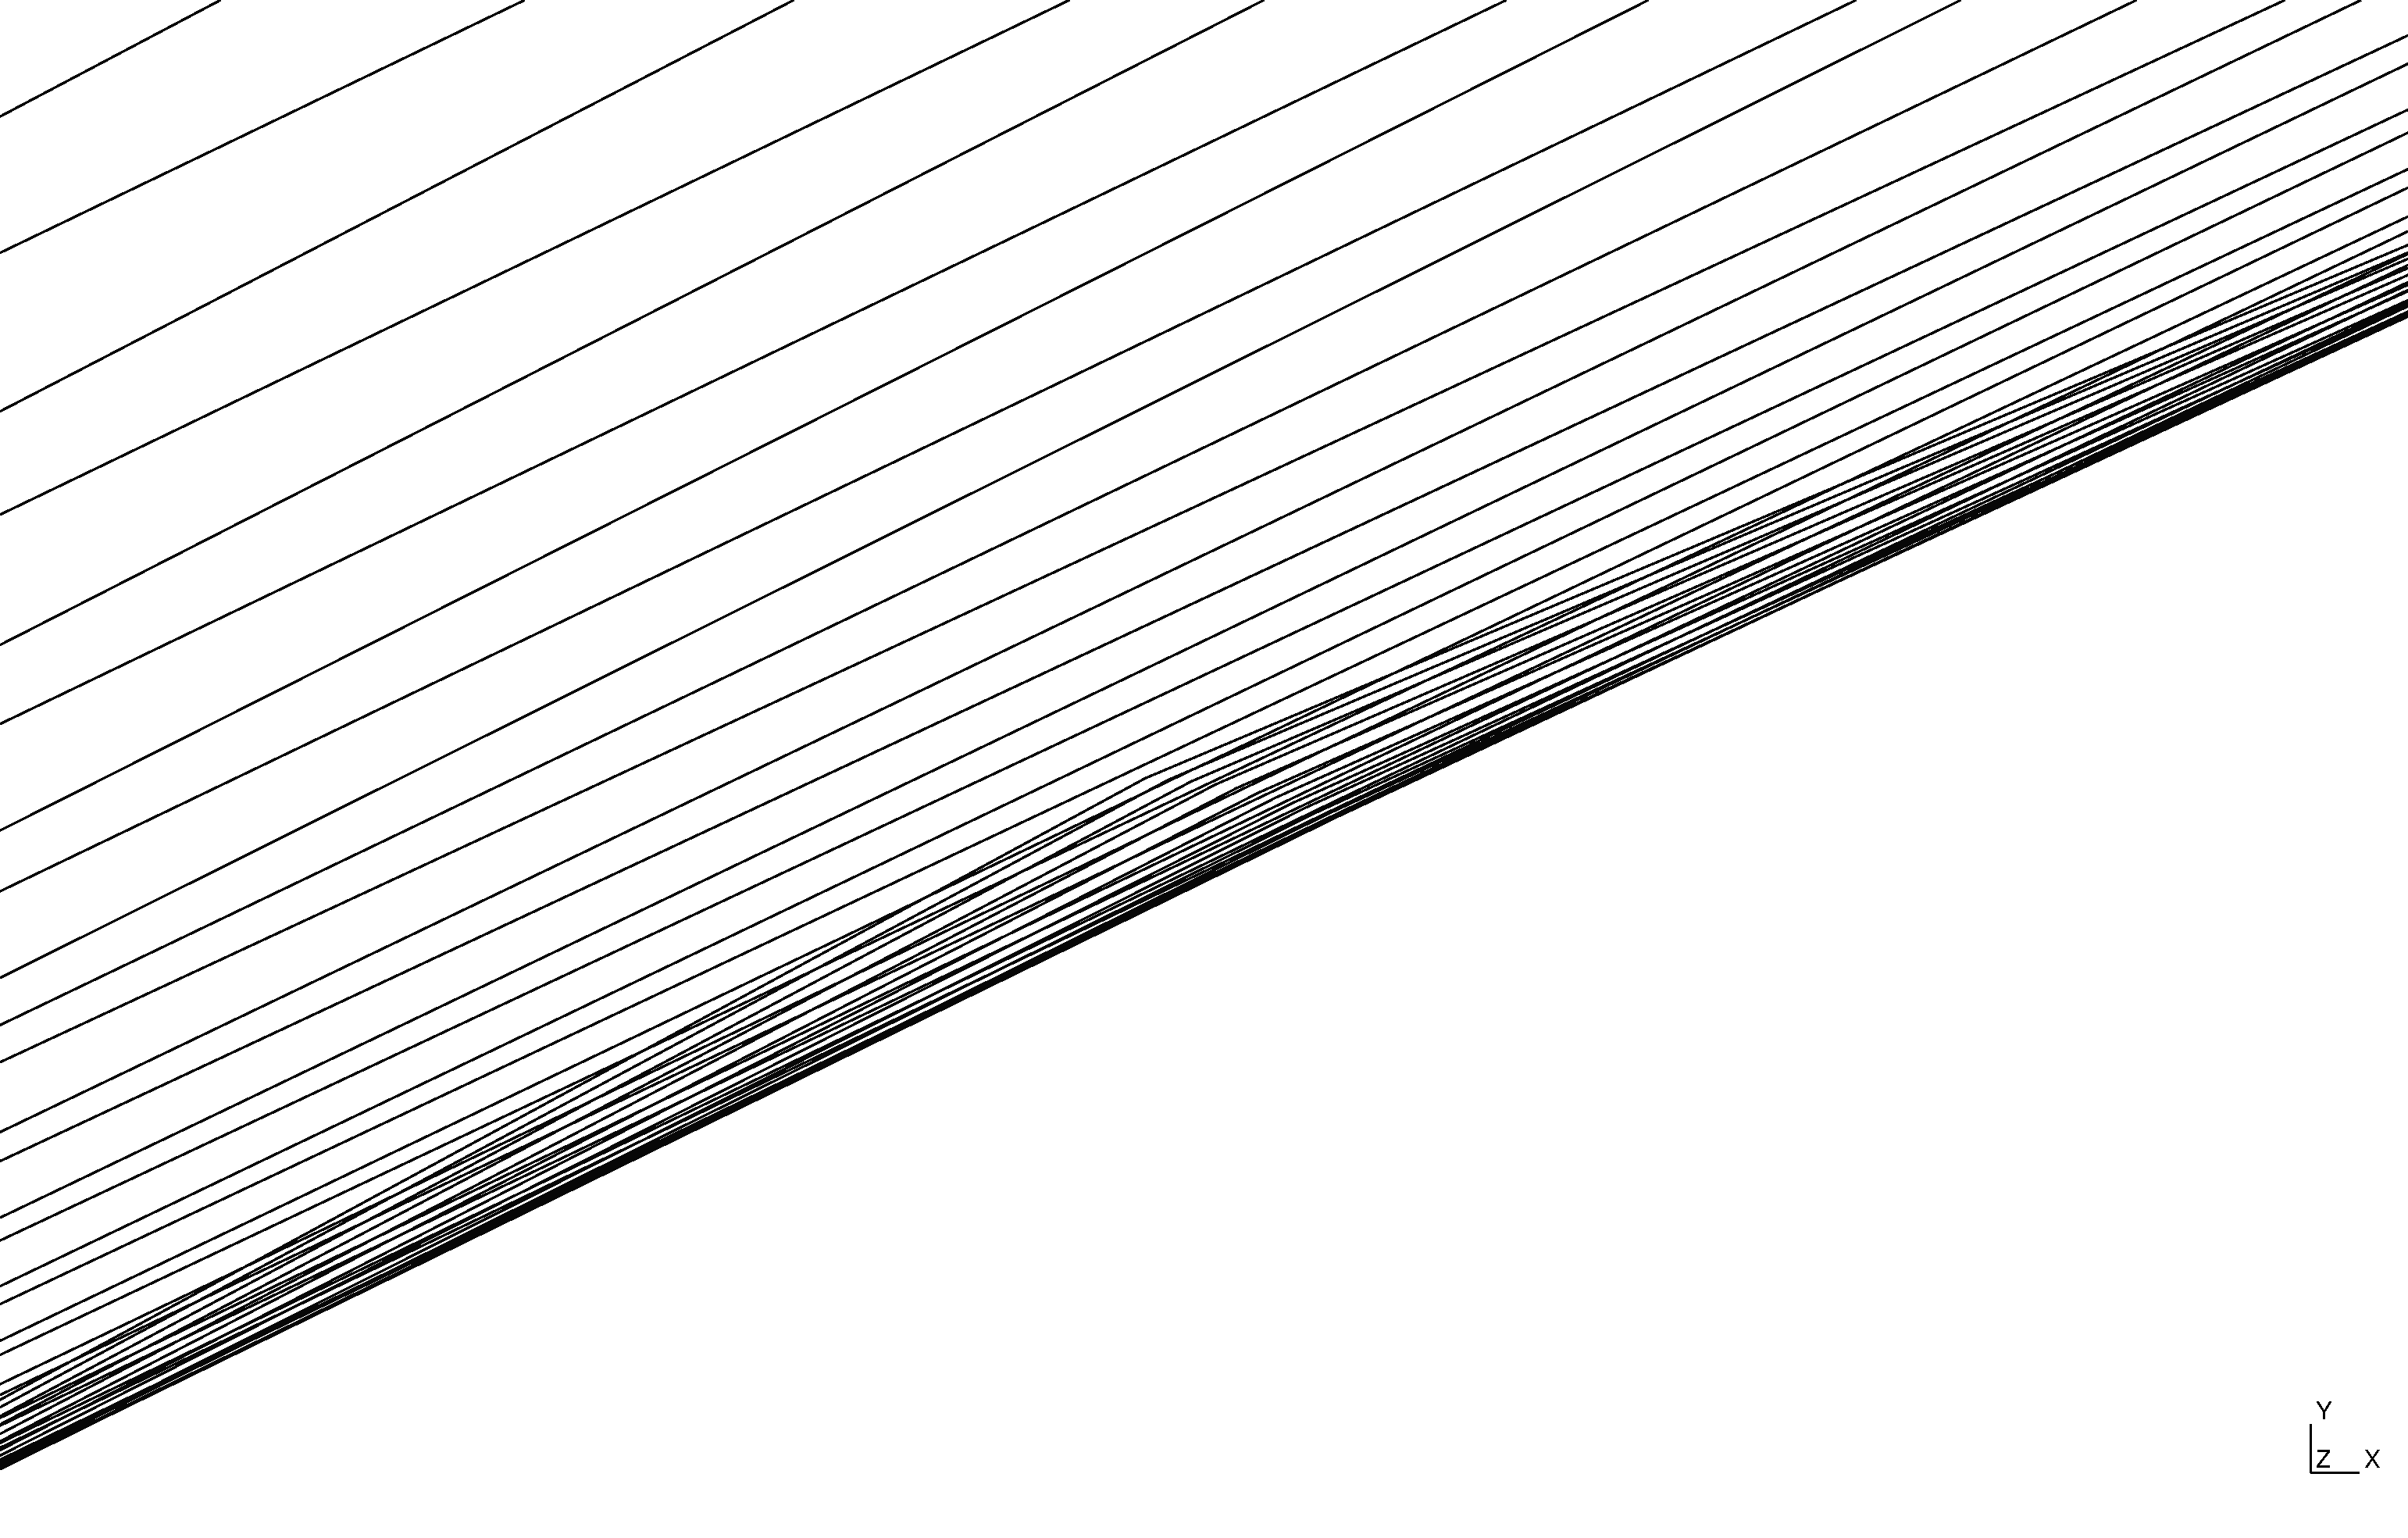
\includegraphics[width=200.0pt]{3comp-elast-vzoomedblk.pdf}
 	}
 	\subfloat{
 		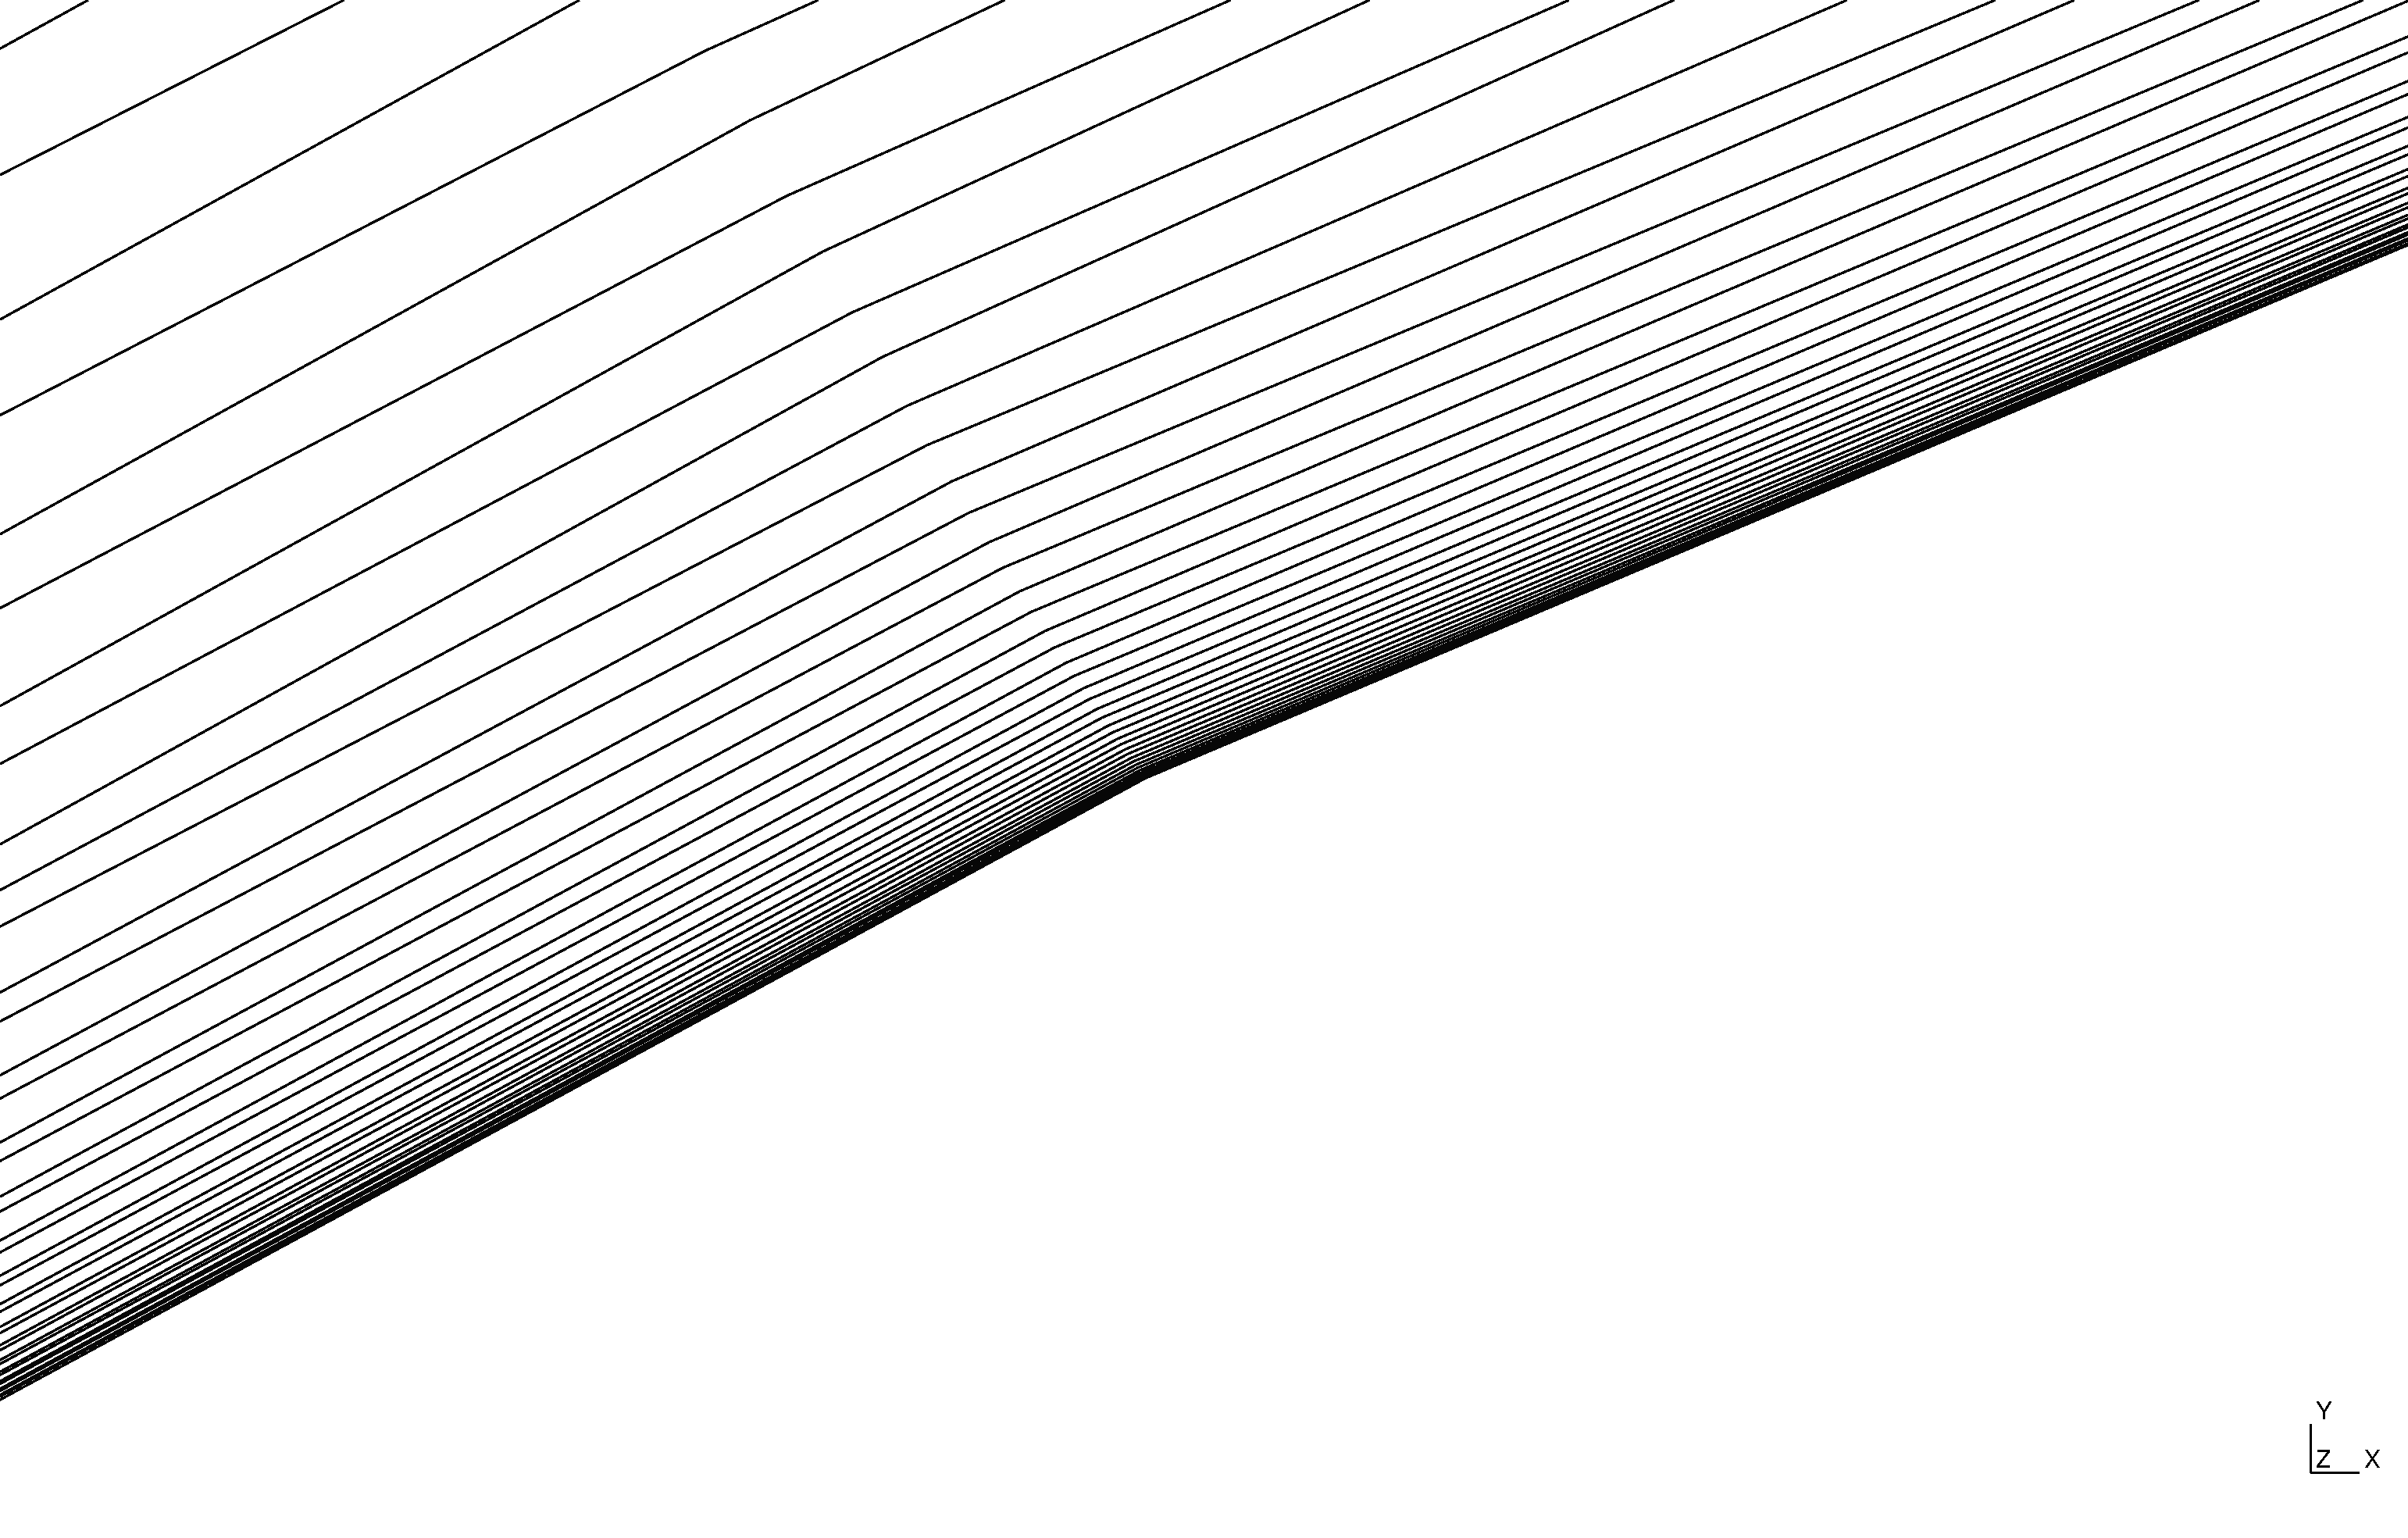
\includegraphics[width=200.0pt]{3comp-rbf-vzoomedblk.pdf}
 	}
 	\caption{Portion of quadratic viscous mesh for multi-element airfoil, showing a boundary face in the flap, generated by linear elasticity (left) and RBF (right) methods. Both are zoomed to for a clearer view.}
 	\label{fig:tangled2}
 \end{figure}
 
 In figures \ref{fig:tangled1} and \ref{fig:tangled2}, the first mesh is tangled; even though the nodes are being moved, they are not being moved far enough. It is clear that simple linear elasticity is not enough for curved mesh generation - we get negative Jacobians in several near-boundary elements for many curved boundary faces. However, the RBF method is satisfactory, with a scaled minimum Jacobian range of 0.64 to 1.0 throughout the mesh (figure \ref{fig:rbf-jacobians}). As explained earlier, we see that the elements very close to the boundary deform very little - they have scaled Jacobian nearly 1.0. As we go further from the boundary, the Jacobian drops to a minimum and then rises again to 1.0 at a distance that approximately equals the support radius.
 
 \begin{figure}
 	\centering
 	\includegraphics[width=400pt,scale=0.5]{3comp-rbf-zoomed-jacobians2.png}
 	\caption{Minimum scaled Jacobian over each element for mesh generated by RBF interpolation. (The mesh is actually curved, though the graphics of Gmsh ignore that.)}
 	\label{fig:rbf-jacobians}
 \end{figure}